\section*{4-bens møbel med skuffe}
Formålet med projektet er at illustrere relevante færdigheder, tilegnet på
snedkeruddannelsens grundforløb, KTS.
Projektet omfatter blandt andet; design og arbejdstegning i CAD program
(\texttt{SolidWorks}), procesbeskrivelse, skæresedel, bestilling af råtræ uden
overdreven spild, behandling af råtræ, maskin- og hånd-lavede samlinger og finerarbejde.

Projektet er et natbord, inspireret af to lignende projekter fra
\texttt{CITYJOINERY}\nolinebreak \footnote{\texttt{cityjoinery.com}}.

\begin{figure}[htb]
\centering
\fbox{
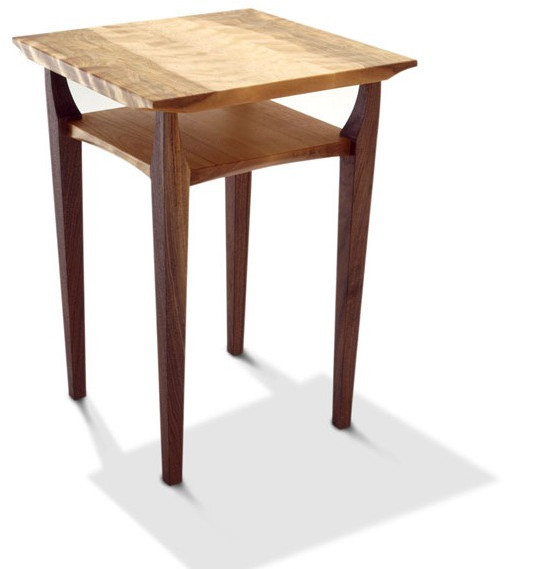
\includegraphics[width=0.4 \textwidth]{imgs/Aspiration-Nightstand-birch.jpg}
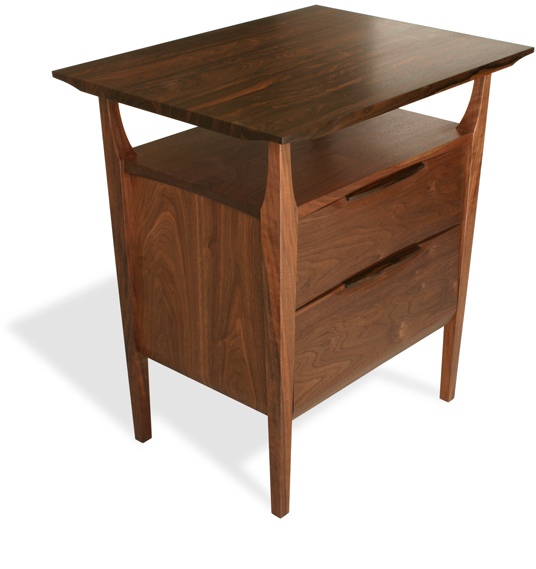
\includegraphics[width=0.4 \textwidth]{imgs/Aspiration-Nightstand-walnut.jpg}
}
\caption{Ende- og nat-bord fra \texttt{CITYJOINERY} i hhv. birk og valnød til
venstre, og valnød til højre.}
\end{figure}

Projektet er et fribensmøbel med sarge, én skuffe hvis top fungerer som hylde,
og en bordplade. Ben, sarge og skuffe front udføres i massiv valnød,
skuffebund, hylde og bordplade, laves af birke-krydsfiner med
valnøddefiner og kantlister, skuffesiderne udføres i elm. Skuffen styres af
flere lister bag sargene, gjort i ahorn.

Natbordets bordplade og hyldetop udføres i krydsfiner, da det er mere stabilt
end massivtræ. Da begge elementer fæstnes til benene, kan de potentielt
skævvride hele møblet, hvis de skulle slå sig med tiden. Brugen af finerede
pladematerialer løser det problem. Alternativt kunne man have brugt samlinger
der giver emnerne mulighed for at forskyde sig i forhold til hinanden.

Valget af elm til skuffesiderne er en smule ukonventionelt. Da skuffen skal
passe ind i møblet, bruger man normalt mere stabile træsorter.
Elm er derudover kendt for at være splintret, med et ujævnt fiber forløb, der kan
virke sløvende på værktøjer. Her bruges elm primært som æstetisk forsøg, da
kerneveddet kan findes i en række forskellige farver. Med henblik på
konstruktion havde ahorn været et bedre valg.

\subsection*{Design valg}
Natbordet har fået flere udskæringer og taperinger, der skal få det til at
fremstå lettere, mindre og mere elegant. Hjørnerne på bordpladen er udskåret på
undersiden, og hvert ben er taperet på de to sider der vender væk fra møblet.
Taperingerne på benene efterlader således indersiderne, ind mod resten af
møblet, som lodrette plan der bruges som reference for skuffen og sargene.
Modsat taperingerne er toppen af benene udskåret fra møblets inderside, hvilket
giver benenes taperede ydersider et øget blikfang. Det giver illusionen af at
benene er montereret skrånende på møblet, selvom indersiderne
er lodrette.
